% !TEX TS-program = pdflatex
% !TEX encoding = UTF-8 Unicode

% This is a simple template for a LaTeX document using the "article" class.
% See "book", "report", "letter" for other types of document.

\documentclass[11pt]{article} % use larger type; default would be 10pt

\usepackage[utf8]{inputenc} % set input encoding (not needed with XeLaTeX)
\usepackage{tikz}
%%% Examples of Article customizations
% These packages are optional, depending whether you want the features they provide.
% See the LaTeX Companion or other references for full information.

%%% PAGE DIMENSIONS
\usepackage{geometry} % to change the page dimensions
\geometry{a4paper} % or letterpaper (US) or a5paper or....
\geometry{margin=0.5in} % for example, change the margins to 2 inches all round
% \geometry{margin=2in} % for example, change the margins to 2 inches all round
% \geometry{landscape} % set up the page for landscape
%   read geometry.pdf for detailed page layout information

\usepackage{graphicx} % support the \includegraphics command and options

% \usepackage[parfill]{parskip} % Activate to begin paragraphs with an empty line rather than an indent

%%% PACKAGES
\usepackage{booktabs} % for much better looking tables
\usepackage{array} % for better arrays (eg matrices) in maths
\usepackage{paralist} % very flexible & customisable lists (eg. enumerate/itemize, etc.)
\usepackage{verbatim} % adds environment for commenting out blocks of text & for better verbatim
\usepackage{subfig} % make it possible to include more than one captioned figure/table in a single float
% These packages are all incorporated in the memoir class to one degree or another...

%%% HEADERS & FOOTERS
\usepackage{fancyhdr} % This should be set AFTER setting up the page geometry
\pagestyle{fancy} % options: empty , plain , fancy
\renewcommand{\headrulewidth}{0pt} % customise the layout...
\lhead{}\chead{}\rhead{}
\lfoot{}\cfoot{\thepage}\rfoot{}

%%% SECTION TITLE APPEARANCE
\usepackage{sectsty}
\allsectionsfont{\sffamily\mdseries\upshape} % (See the fntguide.pdf for font help)
% (This matches ConTeXt defaults)

%%% ToC (table of contents) APPEARANCE
\usepackage[nottoc,notlof,notlot]{tocbibind} % Put the bibliography in the ToC
\usepackage[titles,subfigure]{tocloft} % Alter the style of the Table of Contents
\renewcommand{\cftsecfont}{\rmfamily\mdseries\upshape}
\renewcommand{\cftsecpagefont}{\rmfamily\mdseries\upshape} % No bold!

%%% END Article customizations

%%% The "real" document content comes below...

\title{Week 4 Assignment}
\author{Efeosa Eguavoen - 17324649}
%\date{} % Activate to display a given date or no date (if empty),
         % otherwise the current date is printed 

\begin{document}
\maketitle

\section{(i)}
\subsection{A}
\begin{center}
\includegraphics[scale=0.5]{x1vx2.png}
\end{center}
From the above plot, the data is not linealy seperable so some feature engineering will be required to get the correct decision boundary. The decision boundary I would plot based off the above plot would be some sort of quadratic line. 
\begin{center}
\includegraphics[scale=0.5]{qvalerr.png}
\end{center}
\begin{figure}[h]
\centering
\subfloat[Q =1]{{\includegraphics[width=8cm]{s1.png}}}
\qquad
\subfloat[Q = 2]{{\includegraphics[width=8cm]{s2.png}}}
\qquad
\subfloat[Q = 6]{{\includegraphics[width=8cm]{s3.png}}}
\qquad
\end{figure}
To select the correct order polynomial to use for my model, I started by looking at my graph to get an estimate of the order of polynomial that would be required to get the best decision boundary. From the first graph, I knew that it would at least need to be quadratic to I scanned a range of values between 1 and 6 as having too high an order of polynomials would lead to having too many features that would be unnecessary.I used K=10 for Kfold cross validation as my dataset was sufficiently large I could use a larger number of K. From the above graph, we can see that when Q = 2 and when Q =6 the mean error is lowest. I went with Q=2 as it's better to keep the model as simple as possible. Above I've also plotted the prediction vs training for different Q values. We can clearly see when Q =1 the data on the bottom right and bottom left corner of the graph has been misclassified. In comparison, when Q =2 and when Q=6 we've gotten much better predictions and much less data has been misclassified. The difference between Q=2 and Q=6 is very little based off the graphs.  \\ To get the above graphs I got a range of values for Q and stored them in a list. From there I iterated over the list and created additional features to the Qth power. I trained Logistic Regression models with default C value. Following this I graphed the mean error vs Q and graphed certain predictions for different Q values. 
\begin{verbatim}
def L1Logger():
    q_vals = [f for f in range(1, 20)]
    mean_list = []
    variance_list = []
    for i in q_vals:
        p = PolynomialFeatures(i).fit(df[['x1', 'x2']])
        features = pd.DataFrame(p.transform(df[['x1', 'x2']]), columns=p.get_feature_names(df.columns))
        kf = KFold(n_splits=10)
        error_list = []
        for train, test in kf.split(features):
            x_train, x_test = features.loc[train], features.loc[test]
            y_train, y_test = df.loc[train, 'label'], df.loc[test, 'label']
            model = LogisticRegression(penalty='l1', solver='liblinear')
            model.fit(x_train.values, y_train.values)
            pred = model.predict(x_test)
            error_list.append(mean_squared_error(y_test.values, pred))
\end{verbatim}
\newpage
\begin{figure}[h]
\centering
\subfloat[]{{\includegraphics[width=8cm]{c1.png}}}
\qquad
\subfloat[]{{\includegraphics[width=8cm]{c2.png}}}
\qquad
\subfloat[]{{\includegraphics[width=8cm]{c3.png}}}
\qquad
\subfloat[]{{\includegraphics[width=8cm]{c4.png}}}
\end{figure}
To select the correct value of C for an L1 penalty, I used a range of values of C between 0 and 100 initially to get wide enough spread to select the optimal value of C. From there I reduced the range of values further and further to get the best value of C versus the mean error. From the above graph, C = 0.15 is the optimal value to use for the model as it reduces the error down the most. Higher values of C seem to keep the error around roughly the same value so I just went with the smaller value for simplicity. 
I used a previously selected value of Q and then tried to get the best C value based off the value of Q I selected.
\begin{verbatim}
def c_val():
    p = PolynomialFeatures(2).fit(df[['x1', 'x2']])
    features = pd.DataFrame(p.transform(df[['x1', 'x2']]), columns=p.get_feature_names(df.columns))
    c_vals = np.linspace(0.001, 100, num=50)
    mean_list = []
    std_list = []
    kf = KFold(n_splits=10)
    for i in c_vals:
        error_list = []
        printed = True
        for train, test in kf.split(df):
            x_train, x_test = df.loc[train, ['x1', 'x2']], df.loc[test , ['x1', 'x2']]
            y_train, y_test = df.loc[train, 'label'], df.loc[test, 'label']
            model = LogisticRegression(penalty='l1', solver='liblinear', C=i)
            model.fit(x_train, y_train)
            if printed:
                print(model.intercept_, model.coef_)
                printed = False
            pred = model.predict(x_test)
            error_list.append(mean_squared_error(y_test, pred))
\end{verbatim}

\subsection{B}
\begin{figure}[h]
\centering
\subfloat[K- Large Range]{{\includegraphics[width=8cm]{k1.png}}}
\qquad
\subfloat[K - Small Range]{{\includegraphics[width=8cm]{k2.png}}}
\qquad
\end{figure}
To select a value for K, I first did some research online about guidelines for calculating K. From what I read, I saw k=sqrt(n). I used this as a baseline for the range of values to search over, so I searched between 1 and 100 initially and from there reduced the range down further. I used cross validation for each value of K, with a k value of k=10. Based on the graphs, above, K = 3 is the optimum value of K to use for the given dataset. The mean error when K = 3 is lowest other than when K = 15 which also has a low error rate. Choosing K = 3 is best as it keeps the model simpler.\\
To select K, I first created a list of K values, using odd values of K. I iterated over the list and fitted models for each value. I then got the error and std deviation and plotted vs K.
\begin{verbatim}
def Knn():
    mean_list = []
    std_list = []
    kf = KFold(n_splits=10)
    k_vals = [x for x in range(150) if x % 2 != 0 and x > 80]
    # p = PolynomialFeatures(2).fit(df[['x1', 'x2']])
    # features = pd.DataFrame(p.transform(df[['x1', 'x2']]), columns=p.get_feature_names(df.columns))
    for k in k_vals:
\end{verbatim}
\subsection{C}
Logistic Model: 
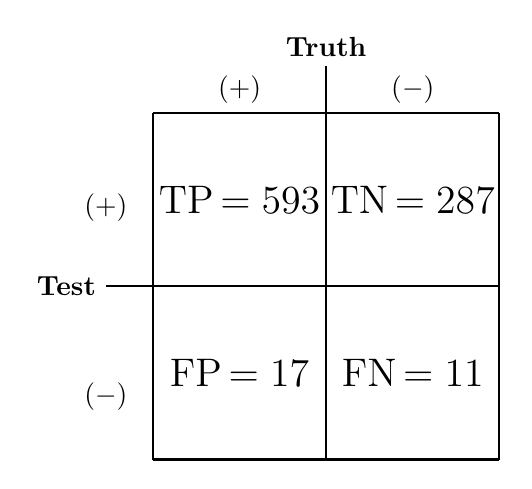
\begin{tikzpicture}[scale=2] %font=\scriptsize
    % Draw Basic Box
    \draw[thick] (0,0) -- (2.2,0);
    \draw[thick] (0,0) -- (0, 2.2);
    \draw[thick] (2.2,2.2) -- (2.2, 0);
    \draw[thick] (2.2,2.2) -- (0, 2.2);

    % Draw Box Ticks
    \draw[thick] (-0.3, 1.1) -- (2.2, 1.1);
    \draw[thick] (1.1, 0) -- (1.1, 2.5);

    % Box Labels
    % -- left side
    \coordinate[label=left:($+$)] (p1) at (-0.1,1.6);
    \coordinate[label=left:($-$)] (p2) at (-0.1,0.4);

    % -- top side
    \coordinate[label=above:($+$)] (p3) at (0.55, 2.2);
    \coordinate[label=above:($-$)] (p4) at (1.65, 2.2);

    % -- overall headers
    \coordinate[label=above:\textbf{Truth}] (p5) at (1.1, 2.5);
    \coordinate[label=left:\textbf{Test}] (p6) at (-0.3, 1.1);

    % Category Values
    \coordinate[label={\Large TP$\,=593$}] (TP) at (0.55, 1.50);
    \coordinate[label={\Large TN$\,=287$}] (FP) at (1.65, 1.50);
    \coordinate[label={\Large FP$\,=17$}] (FN) at (0.55, 0.40);
    \coordinate[label={\Large FN$\,=11$}] (TN) at (1.65, 0.40);
\end{tikzpicture}
KNN Model: 
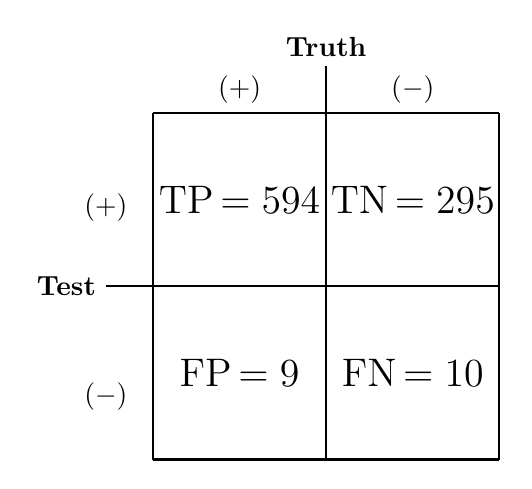
\begin{tikzpicture}[scale=2] %font=\scriptsize
    % Draw Basic Box
    \draw[thick] (0,0) -- (2.2,0);
    \draw[thick] (0,0) -- (0, 2.2);
    \draw[thick] (2.2,2.2) -- (2.2, 0);
    \draw[thick] (2.2,2.2) -- (0, 2.2);

    % Draw Box Ticks
    \draw[thick] (-0.3, 1.1) -- (2.2, 1.1);
    \draw[thick] (1.1, 0) -- (1.1, 2.5);

    % Box Labels
    % -- left side
    \coordinate[label=left:($+$)] (p1) at (-0.1,1.6);
    \coordinate[label=left:($-$)] (p2) at (-0.1,0.4);

    % -- top side
    \coordinate[label=above:($+$)] (p3) at (0.55, 2.2);
    \coordinate[label=above:($-$)] (p4) at (1.65, 2.2);

    % -- overall headers
    \coordinate[label=above:\textbf{Truth}] (p5) at (1.1, 2.5);
    \coordinate[label=left:\textbf{Test}] (p6) at (-0.3, 1.1);

    % Category Values
    \coordinate[label={\Large TP$\,=594$}] (TP) at (0.55, 1.50);
    \coordinate[label={\Large TN$\,=295$}] (FP) at (1.65, 1.50);
    \coordinate[label={\Large FP$\,=9$}] (FN) at (0.55, 0.40);
    \coordinate[label={\Large FN$\,=10$}] (TN) at (1.65, 0.40);
\end{tikzpicture}\\
Most Common:
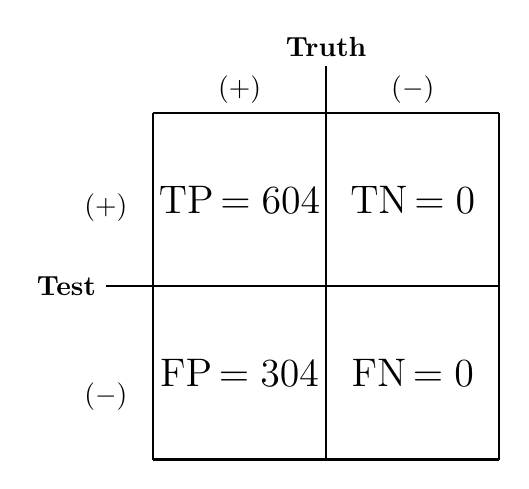
\begin{tikzpicture}[scale=2] %font=\scriptsize
    % Draw Basic Box
    \draw[thick] (0,0) -- (2.2,0);
    \draw[thick] (0,0) -- (0, 2.2);
    \draw[thick] (2.2,2.2) -- (2.2, 0);
    \draw[thick] (2.2,2.2) -- (0, 2.2);

    % Draw Box Ticks
    \draw[thick] (-0.3, 1.1) -- (2.2, 1.1);
    \draw[thick] (1.1, 0) -- (1.1, 2.5);

    % Box Labels
    % -- left side
    \coordinate[label=left:($+$)] (p1) at (-0.1,1.6);
    \coordinate[label=left:($-$)] (p2) at (-0.1,0.4);

    % -- top side
    \coordinate[label=above:($+$)] (p3) at (0.55, 2.2);
    \coordinate[label=above:($-$)] (p4) at (1.65, 2.2);

    % -- overall headers
    \coordinate[label=above:\textbf{Truth}] (p5) at (1.1, 2.5);
    \coordinate[label=left:\textbf{Test}] (p6) at (-0.3, 1.1);

    % Category Values
    \coordinate[label={\Large TP$\,=604$}] (TP) at (0.55, 1.50);
    \coordinate[label={\Large TN$\,=0$}] (FP) at (1.65, 1.50);
    \coordinate[label={\Large FP$\,=304$}] (FN) at (0.55, 0.40);
    \coordinate[label={\Large FN$\,=0$}] (TN) at (1.65, 0.40);
\end{tikzpicture}
Random Model:
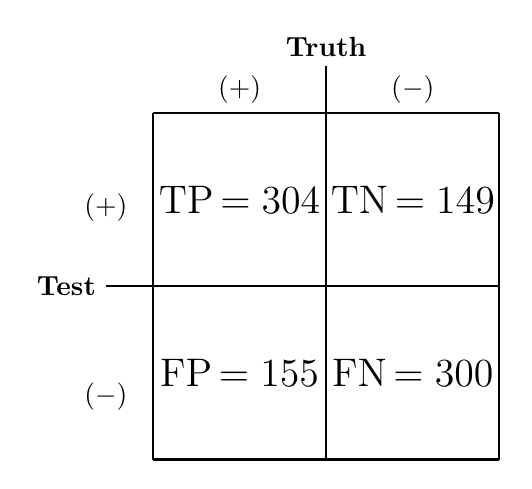
\begin{tikzpicture}[scale=2] %font=\scriptsize
    % Draw Basic Box
    \draw[thick] (0,0) -- (2.2,0);
    \draw[thick] (0,0) -- (0, 2.2);
    \draw[thick] (2.2,2.2) -- (2.2, 0);
    \draw[thick] (2.2,2.2) -- (0, 2.2);

    % Draw Box Ticks
    \draw[thick] (-0.3, 1.1) -- (2.2, 1.1);
    \draw[thick] (1.1, 0) -- (1.1, 2.5);

    % Box Labels
    % -- left side
    \coordinate[label=left:($+$)] (p1) at (-0.1,1.6);
    \coordinate[label=left:($-$)] (p2) at (-0.1,0.4);

    % -- top side
    \coordinate[label=above:($+$)] (p3) at (0.55, 2.2);
    \coordinate[label=above:($-$)] (p4) at (1.65, 2.2);

    % -- overall headers
    \coordinate[label=above:\textbf{Truth}] (p5) at (1.1, 2.5);
    \coordinate[label=left:\textbf{Test}] (p6) at (-0.3, 1.1);

    % Category Values
    \coordinate[label={\Large TP$\,=304$}] (TP) at (0.55, 1.50);
    \coordinate[label={\Large TN$\,=149$}] (FP) at (1.65, 1.50);
    \coordinate[label={\Large FP$\,=155$}] (FN) at (0.55, 0.40);
    \coordinate[label={\Large FN$\,=300$}] (TN) at (1.65, 0.40);
\end{tikzpicture}\\
Logistic Accuracy, Precision: 0.97, 0.97\\
KNN Accuracy, Precision: 0.98, .99\\
Most Common Accuracy, Precision: 0.67, 0.67\\
Random Accuracy, Precision: 0.5, .66 \\
To get the confusion matricies, I made predictions for each of my final  models, then used the confusion matrix function from sci-kit learn. \begin{verbatim}
p = PolynomialFeatures(1).fit(df[['x1', 'x2']])
    features = pd.DataFrame(p.transform(df[['x1', 'x2']]), columns=p.get_feature_names(df.columns))
    lin_model = LogisticRegression(penalty='l1', solver='liblinear', C=0.005).fit(df[['x1', 'x2']], df['label'])
    Knn_model = KNeighborsClassifier(n_neighbors=95, weights='uniform').fit(df[['x1', 'x2']], df['label'])
    vals = [-1, 1]
    most_common = []
    random = rand.choices(vals, k=1803)
    for s in range(1803):
        most_common.append(1)
    models = [lin_model.predict(df[['x1', 'x2']]), Knn_model.predict(df[['x1','x2']]), most_common, random]
    ys = [lin_model.predict_proba(df[['x1', 'x2']])[:, 1], Knn_model.predict_proba(df[['x1','x2']])[:, 1]]
    matrixes = []
    for i in models:
        print(confusion_matrix(df['label'], i))
\end{verbatim}
\subsection{D}
\begin{center}
\includegraphics[scale=0.5]{roc2.png}
\end{center}
We can see in the above graph that our KNN classifier and the Logistic Regression classifier perform nearly identically, both almost reaching the ideal, with the curves almost reaching the top left corner. \\ To get the above graphs, I got the predicted probabilities and then put that against the true values of the label in the roc function. I then plotted the graphs. \begin{verbatim}
ys = [lin_model.predict_proba(df[['x1', 'x2']])[:, 1], Knn_model.predict_proba(df[['x1','x2']])[:, 1]]
rocs = []
    for i in ys:
        fpr,tpr,threshold = roc_curve(df['label'], i)
        rocs.append((fpr,tpr))
\end{verbatim}
\subsection{E}
From the confusion matrices in (c), and the precision and accuracy values, we can see that our Logistic Regression classifier and K-nearest Neighbours classifier both perform very similarly, with the accuracy and precision scores of both have negligible difference between the 2. Both Classifier outperform our baseline models, with the random model being the worst of all our models. The model that predicted that predicted the most common class was more successful than the random model, but when compared to our KNN model or the Logistic Regression model, it performed much worse. From the ROC curves, we can see both our KNN model and Logistic Regression model have curves that are very close to the top left of the grap, with the difference between the two being almost nothing. The AUC of the 2 models is also very similar with the KNN model having a slightly higher AUC. Compared to our baselines on the graph, they both out perform both baselines significantly. \\
Our KNN model performs the best overall out of all our models, with the highest accuracy and the highest precision when classifying, meaning it misclassified the data points the least within those data points it got right. I would recommend using KNN over Logistic Regression for this dataset as the dataset is relatively small so using KNN isn't too intensive, also it performs slightly better than Logistic Regression and also requires much less tuning of hyper parameters with choosing K the only parameter we have to choose.
\newpage
\section{(ii)}
\subsection{A}
\begin{center}
\includegraphics[scale=0.5]{xvx.png}
\end{center}
To start with this dataset, I first plotted the data to see if there was any sort of trends to get an idea of what range of values Q might be in. From the data, there seems to be no clear distinction between the 2 classes. The dataset is also not linearly separable.
\begin{center}
\includegraphics[scale=0.5]{j1.png}
\end{center}

As there was no real trends in the data to select Q from, I just used a large range of values, between 1 and 15. From the above plot, we can see there's no difference for different values of Q, with each value producing a similar result. Due to this fact, I kept Q as 1 as using a higher value of Q didn't produce better results. \\
I plotted the predictions of some of the different q values and as we can see there's no difference between the graphs.
\begin{figure}[h]
\centering
\subfloat[Q =1]{{\includegraphics[width=8cm]{j2.png}}}
\qquad
\subfloat[Q = 2]{{\includegraphics[width=8cm]{j3.png}}}
\qquad
\subfloat[Q = 6]{{\includegraphics[width=8cm]{j4.png}}}
\qquad
\end{figure}
\clearpage
\begin{figure}[h]
\centering
\subfloat[]{{\includegraphics[width=6cm]{f1.jpg}}}
\qquad
\subfloat[]{{\includegraphics[width=6cm]{f2.jpg}}}
\qquad
\subfloat[]{{\includegraphics[width=6cm]{f3.jpg}}}
\qquad
\subfloat[]{{\includegraphics[width=6cm]{f4.png}}}
\qquad
\end{figure}
To Select C I started with a large range of values and then from there narrowed in. Using an L1 penalty, my value of C was very small as I only had 2 feature to use as I kept Q =1. From the data, I let C = 0.005 as it kept the error at it's lowest. Higher values gave the same error so I just used the lowest value possible.
\subsection{B}
\begin{figure}[h]
\centering
\subfloat[]{{\includegraphics[width=8cm]{k3.jpg}}}
\qquad
\subfloat[]{{\includegraphics[width=8cm]{k4.jpg}}}
\qquad
\end{figure}
Using a similar methodology as earlier, I used a range of values between 1 and 150 to get the best value of K. From the above graphs, we can see that the mean error improves as K increase, this could possibly due to the nature of the data being so randomly distributed. From graph b, it seems that K =95 seems to be the optimal solution.
\subsection{C}
Logistic Model: 
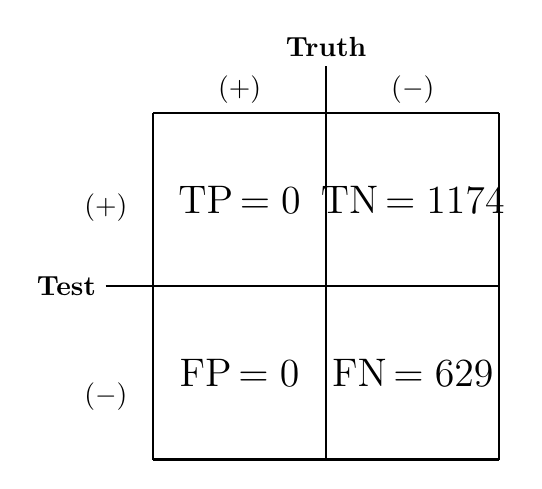
\begin{tikzpicture}[scale=2] %font=\scriptsize
    % Draw Basic Box
    \draw[thick] (0,0) -- (2.2,0);
    \draw[thick] (0,0) -- (0, 2.2);
    \draw[thick] (2.2,2.2) -- (2.2, 0);
    \draw[thick] (2.2,2.2) -- (0, 2.2);

    % Draw Box Ticks
    \draw[thick] (-0.3, 1.1) -- (2.2, 1.1);
    \draw[thick] (1.1, 0) -- (1.1, 2.5);

    % Box Labels
    % -- left side
    \coordinate[label=left:($+$)] (p1) at (-0.1,1.6);
    \coordinate[label=left:($-$)] (p2) at (-0.1,0.4);

    % -- top side
    \coordinate[label=above:($+$)] (p3) at (0.55, 2.2);
    \coordinate[label=above:($-$)] (p4) at (1.65, 2.2);

    % -- overall headers
    \coordinate[label=above:\textbf{Truth}] (p5) at (1.1, 2.5);
    \coordinate[label=left:\textbf{Test}] (p6) at (-0.3, 1.1);

    % Category Values
    \coordinate[label={\Large TP$\,=0$}] (TP) at (0.55, 1.50);
    \coordinate[label={\Large TN$\,=1174$}] (FP) at (1.65, 1.50);
    \coordinate[label={\Large FP$\,=0$}] (FN) at (0.55, 0.40);
    \coordinate[label={\Large FN$\,=629$}] (TN) at (1.65, 0.40);
\end{tikzpicture}
KNN Model: 
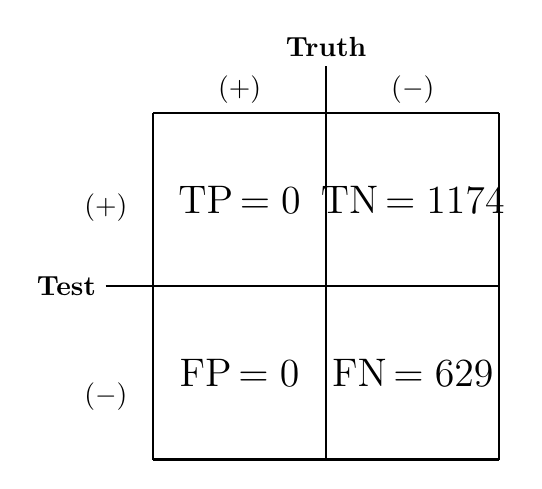
\begin{tikzpicture}[scale=2] %font=\scriptsize
    % Draw Basic Box
    \draw[thick] (0,0) -- (2.2,0);
    \draw[thick] (0,0) -- (0, 2.2);
    \draw[thick] (2.2,2.2) -- (2.2, 0);
    \draw[thick] (2.2,2.2) -- (0, 2.2);

    % Draw Box Ticks
    \draw[thick] (-0.3, 1.1) -- (2.2, 1.1);
    \draw[thick] (1.1, 0) -- (1.1, 2.5);

    % Box Labels
    % -- left side
    \coordinate[label=left:($+$)] (p1) at (-0.1,1.6);
    \coordinate[label=left:($-$)] (p2) at (-0.1,0.4);

    % -- top side
    \coordinate[label=above:($+$)] (p3) at (0.55, 2.2);
    \coordinate[label=above:($-$)] (p4) at (1.65, 2.2);

    % -- overall headers
    \coordinate[label=above:\textbf{Truth}] (p5) at (1.1, 2.5);
    \coordinate[label=left:\textbf{Test}] (p6) at (-0.3, 1.1);

    % Category Values
    \coordinate[label={\Large TP$\,=0$}] (TP) at (0.55, 1.50);
    \coordinate[label={\Large TN$\,=1174$}] (FP) at (1.65, 1.50);
    \coordinate[label={\Large FP$\,=0$}] (FN) at (0.55, 0.40);
    \coordinate[label={\Large FN$\,=629$}] (TN) at (1.65, 0.40);
\end{tikzpicture}\\
Most Common:
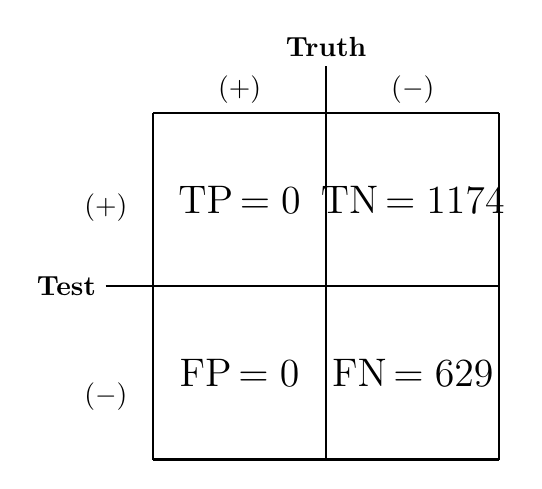
\begin{tikzpicture}[scale=2] %font=\scriptsize
    % Draw Basic Box
    \draw[thick] (0,0) -- (2.2,0);
    \draw[thick] (0,0) -- (0, 2.2);
    \draw[thick] (2.2,2.2) -- (2.2, 0);
    \draw[thick] (2.2,2.2) -- (0, 2.2);

    % Draw Box Ticks
    \draw[thick] (-0.3, 1.1) -- (2.2, 1.1);
    \draw[thick] (1.1, 0) -- (1.1, 2.5);

    % Box Labels
    % -- left side
    \coordinate[label=left:($+$)] (p1) at (-0.1,1.6);
    \coordinate[label=left:($-$)] (p2) at (-0.1,0.4);

    % -- top side
    \coordinate[label=above:($+$)] (p3) at (0.55, 2.2);
    \coordinate[label=above:($-$)] (p4) at (1.65, 2.2);

    % -- overall headers
    \coordinate[label=above:\textbf{Truth}] (p5) at (1.1, 2.5);
    \coordinate[label=left:\textbf{Test}] (p6) at (-0.3, 1.1);

    % Category Values
    \coordinate[label={\Large TP$\,=0$}] (TP) at (0.55, 1.50);
    \coordinate[label={\Large TN$\,=1174$}] (FP) at (1.65, 1.50);
    \coordinate[label={\Large FP$\,=0$}] (FN) at (0.55, 0.40);
    \coordinate[label={\Large FN$\,=629$}] (TN) at (1.65, 0.40);
\end{tikzpicture}
Random Model:
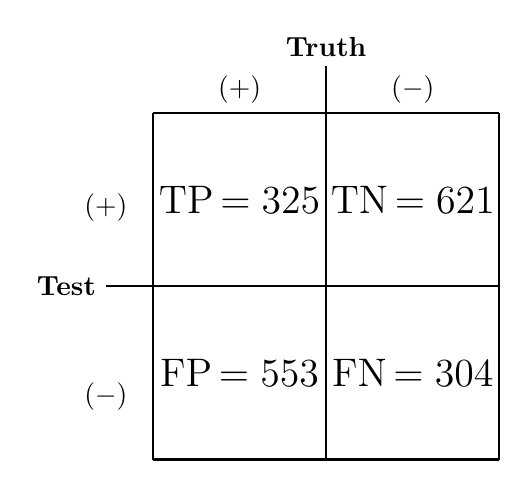
\begin{tikzpicture}[scale=2] %font=\scriptsize
    % Draw Basic Box
    \draw[thick] (0,0) -- (2.2,0);
    \draw[thick] (0,0) -- (0, 2.2);
    \draw[thick] (2.2,2.2) -- (2.2, 0);
    \draw[thick] (2.2,2.2) -- (0, 2.2);

    % Draw Box Ticks
    \draw[thick] (-0.3, 1.1) -- (2.2, 1.1);
    \draw[thick] (1.1, 0) -- (1.1, 2.5);

    % Box Labels
    % -- left side
    \coordinate[label=left:($+$)] (p1) at (-0.1,1.6);
    \coordinate[label=left:($-$)] (p2) at (-0.1,0.4);

    % -- top side
    \coordinate[label=above:($+$)] (p3) at (0.55, 2.2);
    \coordinate[label=above:($-$)] (p4) at (1.65, 2.2);

    % -- overall headers
    \coordinate[label=above:\textbf{Truth}] (p5) at (1.1, 2.5);
    \coordinate[label=left:\textbf{Test}] (p6) at (-0.3, 1.1);

    % Category Values
    \coordinate[label={\Large TP$\,=325$}] (TP) at (0.55, 1.50);
    \coordinate[label={\Large TN$\,=621$}] (FP) at (1.65, 1.50);
    \coordinate[label={\Large FP$\,=553$}] (FN) at (0.55, 0.40);
    \coordinate[label={\Large FN$\,=304$}] (TN) at (1.65, 0.40);
\end{tikzpicture}\\
Logistic Accuracy, Specificity: 0.65, 1\\
KNN Accuracy, Specificity: 0.65, 1\\
Most Common Accuracy, Specificity: 0.65, 1\\
Random Accuracy, Specificity: 0.52,.53  
\subsection{D}
\begin{center}
\includegraphics[scale=0.5]{roc1.png}
\end{center}
\subsection{E}
From our confusion matrices in c, and our ROC curves, we can see that our classifiers both perform very similarly. They perform just slightly better than the random baseline but perform identically to the most common baseline. I think this is due to the fact that given the data is almost completely random with no real way to separate the data, the best course of action would be to predict the most common class, hence our values. I would use either of the classifiers as they both perform the exact same, or I would recommend not using any classifier and just predicting the most common class and not train any model at all as they perform the same regardless.
\section{Code Appendix}
\begin{verbatim}
f = open("ass42.txt", "r")
start = True
data = {'x1': [], 'x2': [], 'label': []}
for i in f:
    if not start:
        i = i.rstrip('\n')
        vals = i.split(",")
        data['x1'].append(float(vals[0]))
        data['x2'].append(float(vals[1]))
        data['label'].append(float(vals[2]))
    else:
        start = False
df = pd.DataFrame(data)
df1 = df[df['label'] == -1]
df2 = df[df['label'] != -1]


def graphs():
    plt.clf()
    plt.scatter(df1['x1'], df1['x2'], marker='+', color='red', label='y = -1')
    plt.scatter(df2['x1'], df2['x2'], marker='o', color='blue', label='y = 1')
    plt.xlabel('X1')
    plt.ylabel('X2')
    plt.title('X1 v X2 with labels for classes')
    plt.legend()
    plt.show()


def L1Logger():
    q_vals = [f for f in range(1, 20)]
    mean_list = []
    variance_list = []
    for i in q_vals:
        p = PolynomialFeatures(i).fit(df[['x1', 'x2']])
        features = pd.DataFrame(p.transform(df[['x1', 'x2']]), columns=p.get_feature_names(df.columns))
        kf = KFold(n_splits=10)
        error_list = []
        plotted = False
        for train, test in kf.split(features):
            x_train, x_test = features.loc[train], features.loc[test]
            y_train, y_test = df.loc[train, 'label'], df.loc[test, 'label']
            model = LogisticRegression(penalty='l1', solver='liblinear')
            model.fit(x_train.values, y_train.values)
            pred = model.predict(x_test)
            error_list.append(mean_squared_error(y_test.values, pred))
            if ((i == 1) or (i == 2) or (i == 6)) and not plotted:
                plt.clf()
                pred = model.predict(features)
                features['pred'] = pred
                i1 = features[features['pred'] == -1]
                i2 = features[features['pred'] != -1]
                plt.scatter(df1['x1'], df1['x2'], marker='+', color='red', label='Class:-1')
                plt.scatter(df2['x1'], df2['x2'], marker='+', color='blue', label='Class:1')
                plt.scatter(i1['x1'], i1['x2'], marker='o', color='green', label='Class:-1', facecolors='none')
                plt.scatter(i2['x1'], i2['x2'], marker='o', color='purple', label='Class:1', facecolors='none')
                plt.xlabel('X1')
                plt.ylabel('X2')
                plt.title(f'Q = {i}')
                plt.legend()
                plt.show()
                plotted = True
        error_list = np.array(error_list)
        mean = error_list.mean()
        mean_list.append(mean)
        var = error_list.var()
        variance_list.append(var)
    plt.clf()
    plt.errorbar(q_vals, mean_list, variance_list, label='Mean Error Line', color='red')
    plt.hlines(y=0, xmin=1, xmax=15, label='Training Data')
    plt.xlabel('Q value')
    plt.ylabel('Mean Error')
    plt.legend()
    plt.show()


def c_val():
    p = PolynomialFeatures(1).fit(df[['x1', 'x2']])
    features = pd.DataFrame(p.transform(df[['x1', 'x2']]), columns=p.get_feature_names(df.columns))
    c_vals = np.linspace(0.001, 100, num=50)
    mean_list = []
    std_list = []
    kf = KFold(n_splits=10)

    for i in c_vals:
        error_list = []
        printed = True
        for train, test in kf.split(df):
            x_train, x_test = df.loc[train, ['x1', 'x2']], df.loc[test , ['x1', 'x2']]
            y_train, y_test = df.loc[train, 'label'], df.loc[test, 'label']
            model = LogisticRegression(penalty='l1', solver='liblinear', C=i)
            model.fit(x_train, y_train)
            if printed:
                print(model.intercept_, model.coef_)
                printed = False
            pred = model.predict(x_test)
            error_list.append(mean_squared_error(y_test, pred))
        error_list = np.array(error_list)
        mean = error_list.mean()
        mean_list.append(mean)
        std = error_list.std()
        std_list.append(std)
    plt.clf()
    plt.errorbar(c_vals, mean_list, yerr=std_list)
    plt.xlabel('C Value')
    plt.ylabel('Mean Error')
    plt.title('C vs Mean Error')
    plt.show()


def Knn():
    mean_list = []
    std_list = []
    kf = KFold(n_splits=10)
    k_vals = [x for x in range(150) if x % 2 != 0 and x > 80]
    # p = PolynomialFeatures(2).fit(df[['x1', 'x2']])
    # features = pd.DataFrame(p.transform(df[['x1', 'x2']]), columns=p.get_feature_names(df.columns))
    for k in k_vals:
        error_list = []
        for train, test in kf.split(df):
            x_train, x_test = df.loc[train, ['x1','x2']], df.loc[test, ['x1','x2']]
            y_train, y_test = df.loc[train, 'label'], df.loc[test, 'label']
            model = KNeighborsClassifier(n_neighbors=k, weights='uniform').fit(x_train, y_train)
            pred = model.predict(x_test)
            error_list.append(mean_squared_error(y_test, pred))
        error_list = np.array(error_list)
        mean = error_list.mean()
        mean_list.append(mean)
        std = error_list.std()
        std_list.append(std)
    plt.clf()
    plt.errorbar(k_vals, mean_list, yerr=std_list)
    plt.xlabel('K')
    plt.ylabel('Mean Error')
    plt.title('K vs Mean Error')
    plt.show()


def conf_matrix():
    p = PolynomialFeatures(1).fit(df[['x1', 'x2']])
    features = pd.DataFrame(p.transform(df[['x1', 'x2']]), columns=p.get_feature_names(df.columns))
    lin_model = LogisticRegression(penalty='l1', solver='liblinear', C=0.005).fit(df[['x1', 'x2']], df['label'])
    Knn_model = KNeighborsClassifier(n_neighbors=95, weights='uniform').fit(df[['x1', 'x2']], df['label'])
    vals = [-1, 1]
    most_common = []
    random = rand.choices(vals, k=1803)
    for s in range(1803):
        most_common.append(1)
    models = [lin_model.predict(df[['x1', 'x2']]), Knn_model.predict(df[['x1','x2']]), most_common, random]
    ys = [lin_model.predict_proba(df[['x1', 'x2']])[:, 1], Knn_model.predict_proba(df[['x1','x2']])[:, 1]]
    matrixes = []
    for i in models:
        print(confusion_matrix(df['label'], i))
    rocs = []
    for i in ys:
        fpr,tpr,threshold = roc_curve(df['label'], i)
        rocs.append((fpr,tpr))
    plt.plot(rocs[0][0],rocs[0][1],color='red',label='linear model')
    plt.plot(rocs[1][0],rocs[1][1],color='blue', label='KNN model')
    plt.plot([0, 1], [0, 1], color='green',linestyle='--', label='Random Classifier')
    plt.xlabel('False Positive Rate')
    plt.ylabel('True Positive Rate')
    plt.legend()
    plt.show()

\end{verbatim}
\end{document}
